\section{Verifizierung Messaufbau}

\subsection{Spannungsmessung}\label{subsec_messu}

\begin{table}[h]
\centering
\begin{tabular}{|r|r|r|r|}
	\hline
	\textbf{Ausgangsspannung} & \textbf{Messwert $messU$} & \textbf{Differenz} & \textbf{Fehler} \\ \hline
	0.0V & 0mV & - & 0.0mV \\ \hline
	1.0V & 202mV & 202mV & -0.3mV \\ \hline
	2.0V & 406mV & 204mV & +1.7mV \\ \hline
	3.0V & 608mV & 202mV & -0.3mV \\ \hline
	4.0V & 811mV & 203mV & +0.7mV \\ \hline
	5.0V & 1013mV & 202mV & -0.3mV \\ \hline
	6.0V & 1216mV & 203mV & +0.7mV \\ \hline
	7.0V & 1418mV & 202mV & -0.3mV \\ \hline
	8.0V & 1621mV & 203mV & +0.7mV \\ \hline
	9.0V & 1824mV & 203mV & +0.7mV \\ \hline
	10.0V & 2026mV & 202mV & -0.3mV \\ \hline
	11.0V & 2228mV & 202mV & -0.3mV \\ \hline
	12.0V & 2430mV & 202mV & -0.3mV \\ \hline
	13.0V & 2632mV & 202mV & -0.3mV \\ \hline
	14.0V & 2834mV & 202mV & -0.3mV \\ \hline
	15.0V & 3036mV & 202mV & -0.3mV \\ \hline
	16.0V & 3239mV & 203mV & +0.7mV \\ \hline
	17.0V & 3441mV & 202mV & -0.3mV \\ \hline
	18.0V & 3644mV & 203mV & +0.7mV \\ \hline
	19.0V & 3845mV & 201mV & -1.3mV \\ \hline
	20.0V & 4048mV & 203mV & +0.7mV \\ \hline
	21.0V & 4251mV & 203mV & +0.7mV \\ \hline
	22.0V & 4454mV & 203mV & +0.7mV \\ \hline
	23.0V & 4657mV & 203mV & +0.7mV \\ \hline
	24.0V & 4860mV & 203mV & +0.7mV \\ \hline
\end{tabular}
\caption{Verifizierung der Messwerte $messU$ des Spannungsteilers.}
\label{tab:messU}
\end{table}

Die Spannung wird mittels eines Spannungsteilers aus zwei Widerstände bemessen. Die Toleranz beider Widerstände beträgt $\pm$ 1\%, im schlechtesten Fall ist ein Widerstand am oberen Ende der Toleranz, der andere am unteren Ende (beispielsweise 39.39k$\Omega$ und 9.9k$\Omega$ anstelle von 39k$\Omega$ und 10k$\Omega$). Der maximal mögliche Fehler beträgt damit 2.02\%. \newline
Um diesen Fehler auszuschliessen, wurde die Spannung am Ausgang des Spannungsteilers bei der grössten und der kleinsten möglichen Ausgangsspannung gemessen und die Differenz als 202.3mV pro V Ausgangsspannungserhöhung bestimmt. Mit den in Tabelle \ref{tab:messU} folgenden Messreihe wurde die Genauigkeit dieser Schaltung verifiziert.

Die Fehler sind sehr klein und gleichen sich zumeist aus. Ausserdem sind die Fehler jeweils deutlich kleiner als die Auflösung des AD-Wandlers des Mikrocontrollers. Die Ausgangsspannung beträgt gemäss obiger Messreihe:
\begin{equation}
	U=\text{Messwert}\cdot 4.938
\label{eq:messreihe_messu}
\end{equation}
Für die Software, in welcher alle Werte in Millivolt betrachtet werden, wird $istU$ mit Formel \ref{eq:messreihe_messu} folgendermassen bestimmt:
\begin{equation}
	istU=messU\cdot\frac{400}{81}
\label{eq:messreihe_messu_sw}
\end{equation}


\subsection{Strommessung}\label{subsec_messi}

\begin{table}[h]%
\centering
\begin{tabular}{|r|r|r|r|}
	\hline
	\textbf{Ausgangsstrom} & \textbf{Messwert $messI$} & \textbf{Differenz} & \textbf{Fehler} \\ \hline
	0.0A & 247mV & - & 247mV \\ \hline
	0.2A & 525mV & 278mV & -3.5mV \\ \hline
	0.4A & 809mV & 284mV & +2.5mV \\ \hline
	0.6A & 1093mV & 284mV & +2.5mV \\ \hline
	0.8A & 1374mV & 281mV & -0.5mV \\ \hline
	1.0A & 1660mV & 286mV & +4.5mV \\ \hline
	1.2A & 1943mV & 283mV & +1.5mV \\ \hline
	1.4A & 2223mV & 280mV & -1.5mV \\ \hline
	1.6A & 2507mV & 284mV & +2.5mV \\ \hline
	1.8A & 2785mV & 278mV & -3.5mV \\ \hline
	2.0A & 3061mV & 276mV & -5.5mV \\ \hline
	2.2A & 3344mV & 283mV & +1.5mV \\ \hline
	2.4A & 3629mV & 285mV & +3.5mV \\ \hline
	2.6A & 3907mV & 278mV & -3.5mV \\ \hline
	2.8A & 4187mV & 280mV & -1.5mV \\ \hline
	3.0A & 4469mV & 282mV & +0.5mV \\ \hline
\end{tabular}
\caption{Verifizierung der Messwerte $messI$ der Strommessung.}
\label{tab:messI}
\end{table}

Die Strommessung beinhaltet Widerstände, Operationsverstärker sowie einen Hallsensor, die allesamt Toleranzen unterworfen sind. Am kritischsten ist dabei sicherlich der Spannungsteiler aus 2x 1k$\Omega$, der für die Subtraktionsschaltung benötigt wird. Bei einer Toleranz von 1\% kann die Spannung dabei 2.5V$\pm$50.5mV betragen. Diese Spannungsdifferenz wird jedoch ebenfalls um den Faktor 7.5 Verstärkt, wodurch der maximale Fehler bereits 378.8mV beträgt, was bei 10bit Auflösung des AD-Wandlers durchaus relevant ist. \newline
Aus diesem Grund wurde eine Messreihe durchgeführt. Dabei wurde die Spannung am Ausgang der Messschaltung zuerst bei minimalem und anschliessend bei maximalem Strom der verfügbaren Stromquelle gemessen. Pro 0.2A mehr Ausgangsstrom sollte die Spannung $messI$ gemäss dieser Messung um 281.5mV zunehmen, ausserdem ist ein Offset von 247mV vorhanden. Diese Werte wurden bis zu einem Maximalstrom von 3.0A in Tabelle \ref{tab:messI} ermittelt.

Die Fehler sind ungefähr gleichmässig verteilt und können mit der Ungenauigkeit der verwendeten Stromquelle erklärt werden. Jedoch sind sie deutlich grösser als beim Spannungsteiler, jedoch noch weit unterhalb der geforderten Genauigkeit. Der Ausgangsstrom beträgt gemäss obiger Messreihe:
\begin{equation}
	I=\frac{Messwert-247mV}{1.407}
\label{eq:messreihe_messi}
\end{equation}
Für die Software, in welcher alle Werte in Millivolt und Milliampere betrachtet werden, wird $istI$ mit Formel \ref{eq:messreihe_messi} folgendermassen bestimmt:
\begin{equation}
	istI=\left(messI-247mV\right)\cdot\frac{2111}{1500}
\label{eq:messreihe_messi_sw}
\end{equation}



\newpage
\section{Reglermessung}\label{ValidMeas}

\begin{table}[h]
\centering

\begin{tabular}{|l|l|l|l|l|l|}
\hline
\multicolumn{1}{|c|}{Vin (V)} & \multicolumn{1}{c|}{Iin (A)} & \multicolumn{1}{c|}{Vout (V)} & \multicolumn{1}{c|}{Iout (I)} & \multicolumn{1}{c|}{Resistance (Ohm)} & \multicolumn{1}{c|}{Effizienz} \\ \hline
24.99                         & 0.009                        & 22.89                         & 0                             & -                                     & -                              \\ \hline
24.98                         & 0.448                        & 20.94                         & 0.461                         & 45.4229935                            & 0.86259543                     \\ \hline
24.98                         & 0.594                        & 20.82                         & 0.621                         & 33.52657                              & 0.87135163                     \\ \hline
24.98                         & 0.855                        & 20.64                         & 0.908                         & 22.7312775                            & 0.87747953                     \\ \hline
24.97                         & 1.055                        & 20.5                          & 1.129                         & 18.1576616                            & 0.87857087                     \\ \hline
24.97                         & 1.303                        & 20.35                         & 1.397                         & 14.5669291                            & 0.87377147                     \\ \hline
24.97                         & 1.451                        & 20.27                         & 1.558                         & 13.0102696                            & 0.87163618                     \\ \hline
24.95                         & 1.744                        & 20.12                         & 1.887                         & 10.6624271                            & 0.87253498                     \\ \hline
24.95                         & 1.86                         & 20.07                         & 2.002                         & 10.024975                             & 0.86582067                     \\ \hline
24.99                         & 2.11                         & 19.85                         & 2.29                          & 8.66812227                            & 0.86207943                     \\ \hline
24.98                         & 2.271                        & 19.88                         & 2.451                         & 8.11097511                            & 0.85891487                     \\ \hline
24.98                         & 2.561                        & 19.73                         & 2.77                          & 7.12274368                            & 0.85428905                     \\ \hline
24.98                         & 2.77                         & 19.63                         & 2.984                         & 6.57841823                            & 0.84653889                     \\ \hline
23.71                         & 2.976                        & 18.37                         & 3.202                         & 5.73703935                            & 0.83361593                     \\ \hline
20.44                         & 2.97                         & 15.33                         & 3.203                         & 4.786138                              & 0.80883838                     \\ \hline
17.96                         & 2.963                        & 13.17                         & 3.189                         & 4.12982126                            & 0.78922768                     \\ \hline
16.7                          & 2.965                        & 12.03                         & 3.171                         & 3.79375591                            & 0.77040785                     \\ \hline
11.86                         & 2.954                        & 7.89                          & 3.108                         & 2.53861004                            & 0.69994326                     \\ \hline
9.85                          & 2.952                        & 6.1                           & 3.079                         & 1.98116272                            & 0.64593221                     \\ \hline
6.75                          & 2.95                         & 3.2                           & 3.056                         & 1.04712042                            & 0.4911086                      \\ \hline
\end{tabular}
\caption{Gemessene Maximalwerte des Reglers}
\label{fig::maxValues}
\end{table}

Diese Werte wurden bei maximaler Spannung gemessen (Spannung am Feedback Pin 0v) und dienen dazu, zu überprüfen ob der Regler für die verlangte Anwendung geeignet ist.
\newpage
\begin{table}[h]
\centering

\label{fig::Res6}
\begin{tabular}{|l|l|l|l|l|l|l|l|l|}
\hline
\multicolumn{1}{|c|}{Vin (V)} & \multicolumn{1}{c|}{Iin (I)} & \multicolumn{1}{c|}{Fb (V)} & \multicolumn{1}{c|}{Vout (V)} & \multicolumn{1}{c|}{Iout (I)} & \multicolumn{1}{c|}{Rippel (mV)} & \multicolumn{1}{c|}{Rippel \%} & \multicolumn{1}{c|}{Resistance Ohm)} & \multicolumn{1}{c|}{Effizienz} \\ \hline
24.99                         & 0.008                        & 2.5                         & 0                             & 0                             & 80                               & -                              & -                                    & -                              \\ \hline
24.98                         & 0.06                         & 2.2                         & 2.109                         & 0.342                         & 580                              & 0.275                          & 6.167                                & 0.481                          \\ \hline
24.96                         & 0.26                         & 1.9                         & 5.083                         & 0.819                         & 500                              & 0.098                          & 6.206                                & 0.641                          \\ \hline
25.03                         & 0.57                         & 1.6                         & 8                             & 1.251                         & 720                              & 0.090                          & 6.395                                & 0.701                          \\ \hline
24.96                         & 0.98                         & 1.3                         & 10.92                         & 1.74                          & 560                              & 0.051                          & 6.276                                & 0.777                          \\ \hline
24.98                         & 1.543                        & 1                           & 13.87                         & 2.26                          & 560                              & 0.040                          & 6.137                                & 0.813                          \\ \hline
24.96                         & 2.21                         & 0.7                         & 16.79                         & 2.7                           & 554                              & 0.033                          & 6.219                                & 0.822                          \\ \hline
24.96                         & 2.902                        & 0.4                         & 19.37                         & 3.125                         & 574                              & 0.030                          & 6.198                                & 0.836                          \\ \hline
24.96                         & 3.004                        & 0.12                        & 19.28                         & 3.221                         & 604                              & 0.031                          & 5.986                                & 0.828                          \\ \hline
\end{tabular}
\caption{Messreihe bei 6 $\Omega$ Lastwiderstand}
\end{table}

\begin{table}[h]
\centering
\begin{tabular}{|l|l|l|l|l|l|l|l|l|}
\hline
Vin (V) & Iin (I) & Fb (V) & Vout (V) & Iout (I) & Rippel (mV) & Rippel \% & Resistance Ohm) & Effizienz \\ \hline
24.97 & 0.008 & 2.5 & 0 & 0 & 0 & - & - & - \\ \hline
24.97 & 0.026 & 2.2 & 2.192 & 0.105 & 139 & 0.063 & 20.88 & 0.355 \\ \hline
24.97 & 0.087 & 1.9 & 5.166 & 0.247 & 315 & 0.061 & 20.91 & 0.587 \\ \hline
24.97 & 0.187 & 1.6 & 8.12 & 0.288 & 371 & 0.046 & 28.19 & 0.501 \\ \hline
24.97 & 0.32 & 1.3 & 11.08 & 0.53 & 382 & 0.034 & 20.91 & 0.735 \\ \hline
24.97 & 0.488 & 1 & 14.14 & 0.675 & 384 & 0.027 & 20.95 & 0.783 \\ \hline
24.97 & 0.676 & 0.7 & 17.08 & 0.817 & 380 & 0.022 & 20.91 & 0.827 \\ \hline
24.97 & 0.884 & 0.4 & 20.07 & 0.959 & 375 & 0.019 & 20.93 & 0.872 \\ \hline
24.97 & 0.919 & 0.12 & 20.51 & 0.98 & 374 & 0.018 & 20.93 & 0.876 \\ \hline
\end{tabular}
\caption{Messreihe bei 20 $\Omega$ Lastwiderstand}
\label{fig::Res20}
\end{table}

\begin{table}[h]
\centering
\begin{tabular}{|l|l|l|l|l|l|l|l|l|}
\hline
\multicolumn{1}{|c|}{Vin (V)} & \multicolumn{1}{c|}{Iin (I)} & \multicolumn{1}{c|}{Fb (V)} & \multicolumn{1}{c|}{Vout (V)} & \multicolumn{1}{c|}{Iout (I)} & \multicolumn{1}{c|}{Rippel (mV)} & \multicolumn{1}{c|}{Rippel \%} & \multicolumn{1}{c|}{Resistance Ohm)} & \multicolumn{1}{c|}{Effizienz} \\ \hline
24.97 & 0.008 & 2.5 & 0 & 0 & 0 & - & - & - \\ \hline
24.99 & 0.155 & 2.2 & 2.069 & 0.682 & 399 & 0.193 & 3.034 & 0.364 \\ \hline
24.93 & 0.482 & 1.9 & 4.863 & 1.642 & 490 & 0.101 & 2.962 & 0.665 \\ \hline
24.92 & 1.134 & 1.6 & 7.71 & 2.624 & 592 & 0.077 & 2.938 & 0.716 \\ \hline
24.93 & 2.014 & 1.3 & 10.52 & 3.6 & 595 & 0.057 & 2.922 & 0.754 \\ \hline
14.54 & 3.074 & 1 & 9.75 & 3.333 & 530 & 0.054 & 2.925 & 0.727 \\ \hline
14.52 & 3.066 & 0.7 & 9.71 & 3.327 & 488 & 0.050 & 2.919 & 0.726 \\ \hline
14.31 & 3.058 & 0.4 & 9.65 & 3.307 & 467 & 0.048 & 2.918 & 0.729 \\ \hline
13.9 & 3.06 & 0.12 & 9.46 & 3.46 & 469 & 0.050 & 2.734 & 0.770 \\ \hline
\end{tabular}
\caption{Messreihe bei 3 $\Omega$ Lastwiderstand}
\label{fig::Res3}
\end{table}

Diese Messungen sollen die Regelung per Feedback Pin überprüfen. Die gemessenen Werte sollten linear zur Spannung am Feedback Pin sein.
\newpage

\section{CAD-Pläne des Gehäuses}\label{cad}
Nachfolgend die CAD-Pläne der Vorderseite (Abbildung \ref{fig:Cad_Vorderseite}), der Rückseite (Abbildung \ref{fig:Cad_Ruckseite}) und der Bodenplatte (Abbildung \ref{fig:Cad_Bodenplatte}) des Gehäuses. Diese Pläne befinden sich ebenfalls als .PDF-Datei und .DXF-Datei auf der CD-ROM (Abschnitt \ref{cd}).

\begin{figure}[h]
	\centering
		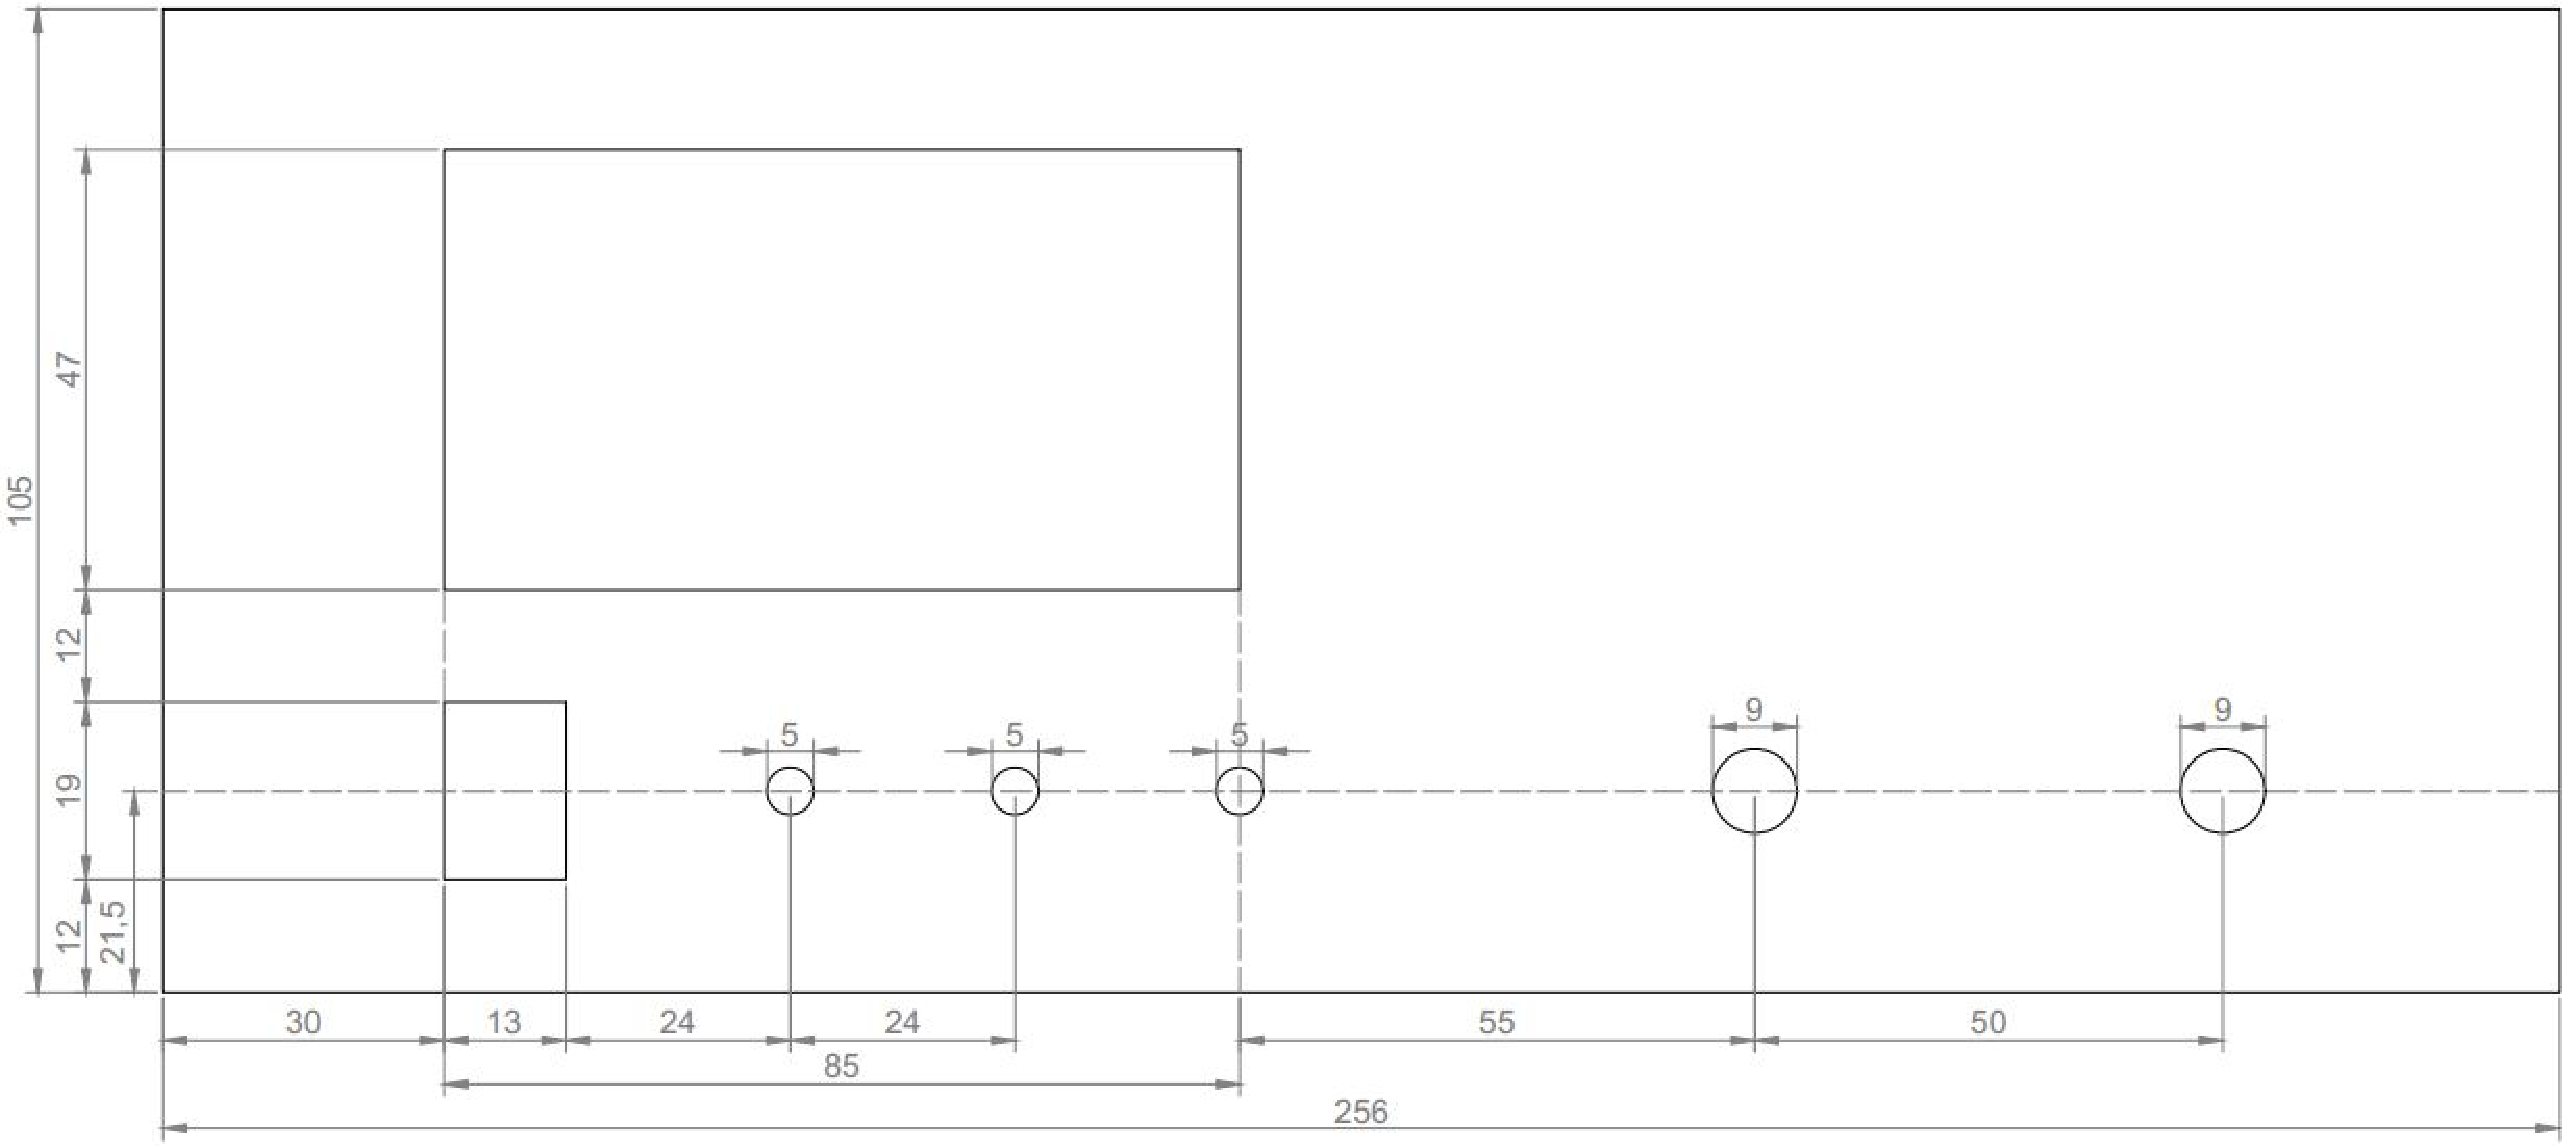
\includegraphics[width=1.00\textwidth]{Cad_Vorderseite.pdf}
	\caption{CAD Zeichnung der Gehäusefront.}
	\label{fig:Cad_Vorderseite}
\end{figure}

\begin{figure}[h]
	\centering
		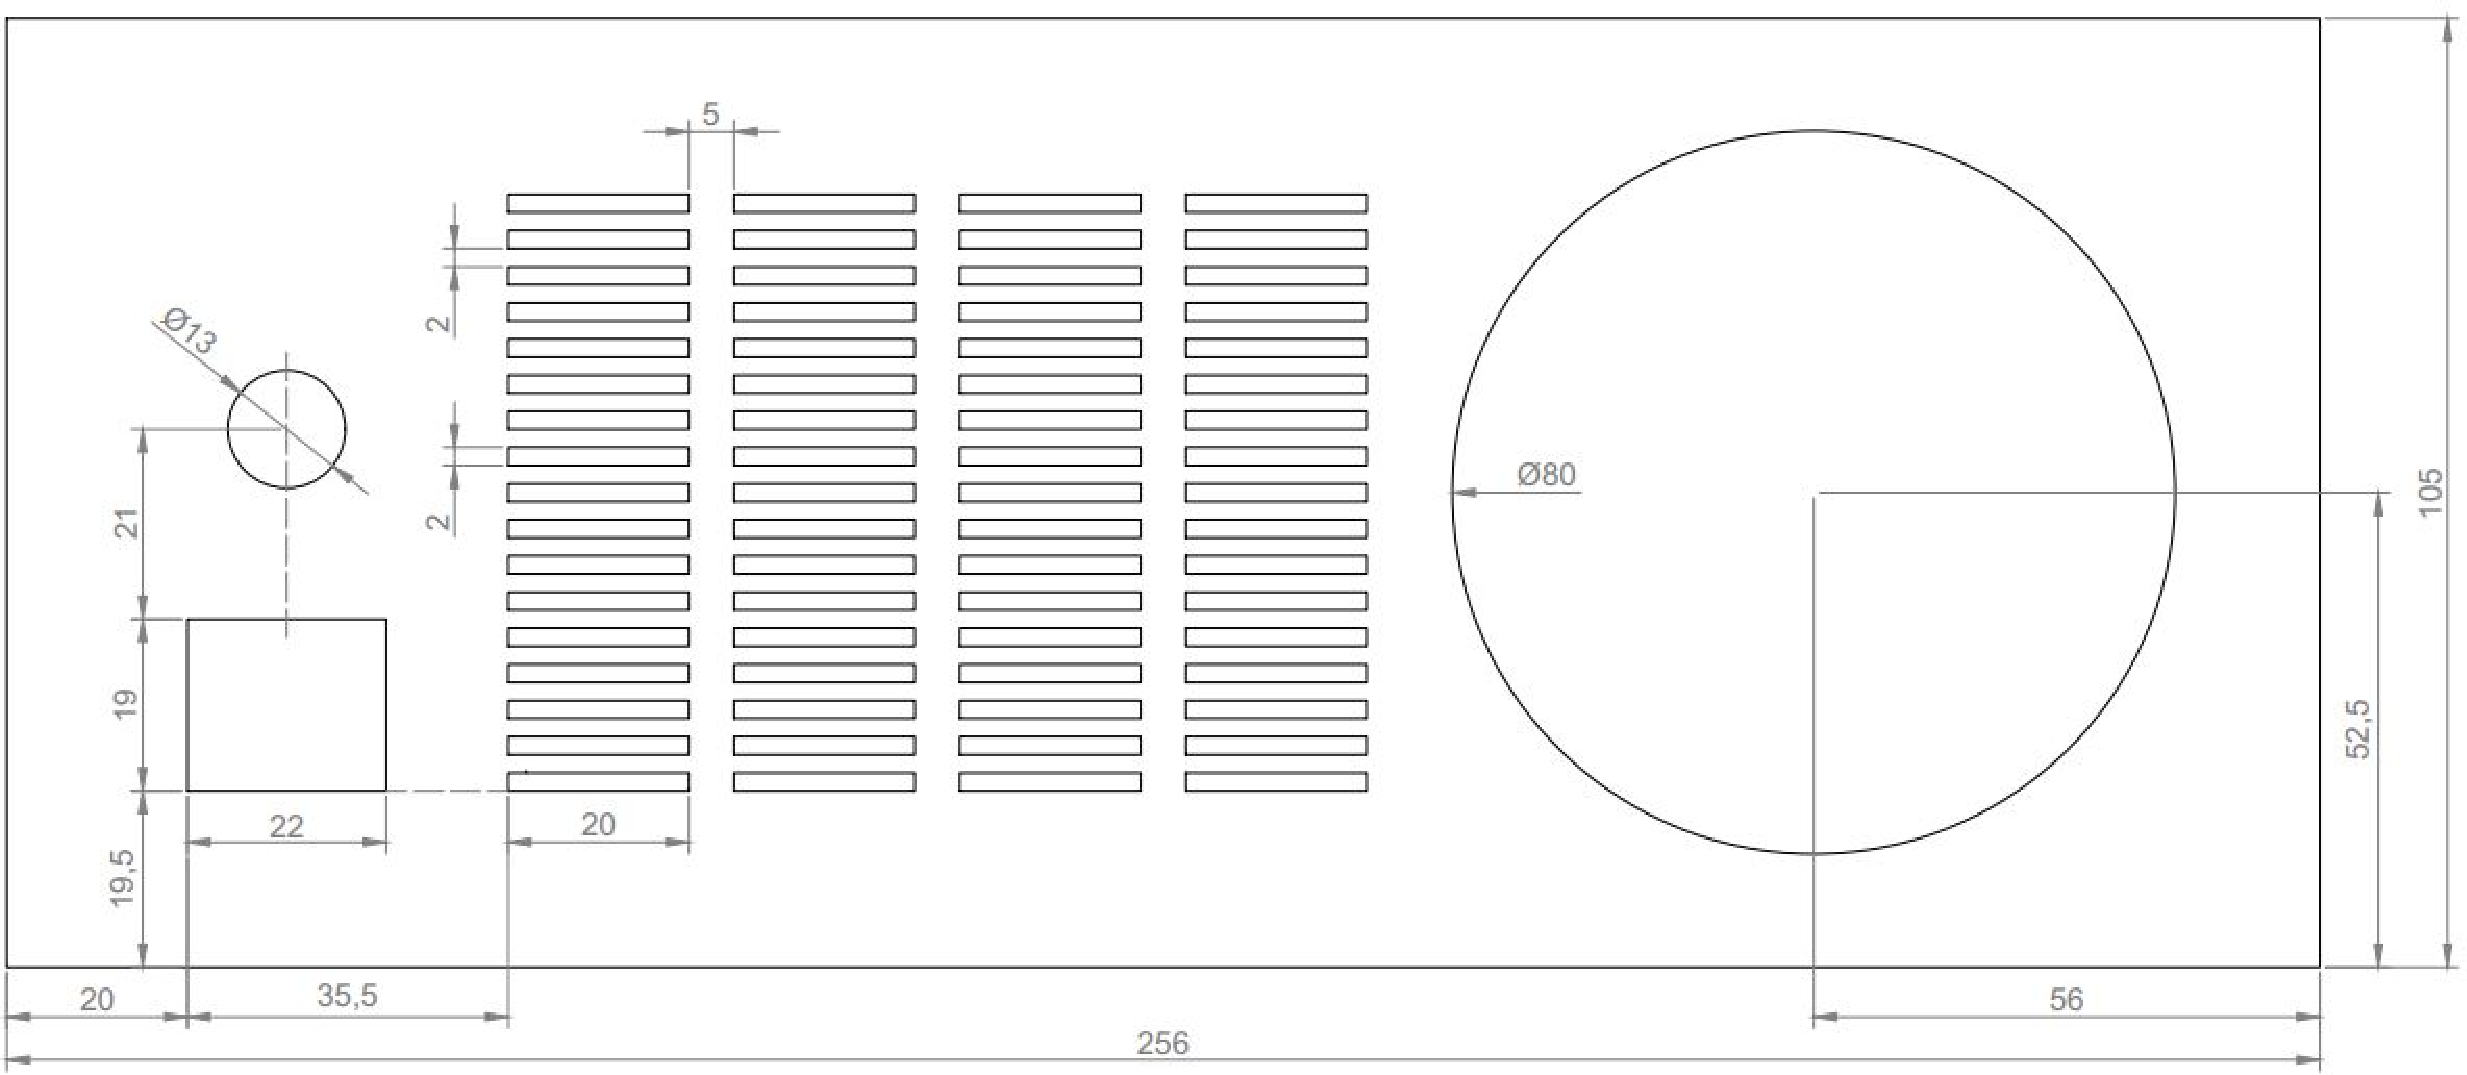
\includegraphics[width=1.00\textwidth]{Cad_Ruckseite.pdf}
	\caption{CAD Zeichnung der Gehäuserückseite.}
	\label{fig:Cad_Ruckseite}
\end{figure}

\begin{figure}[h]
	\centering
		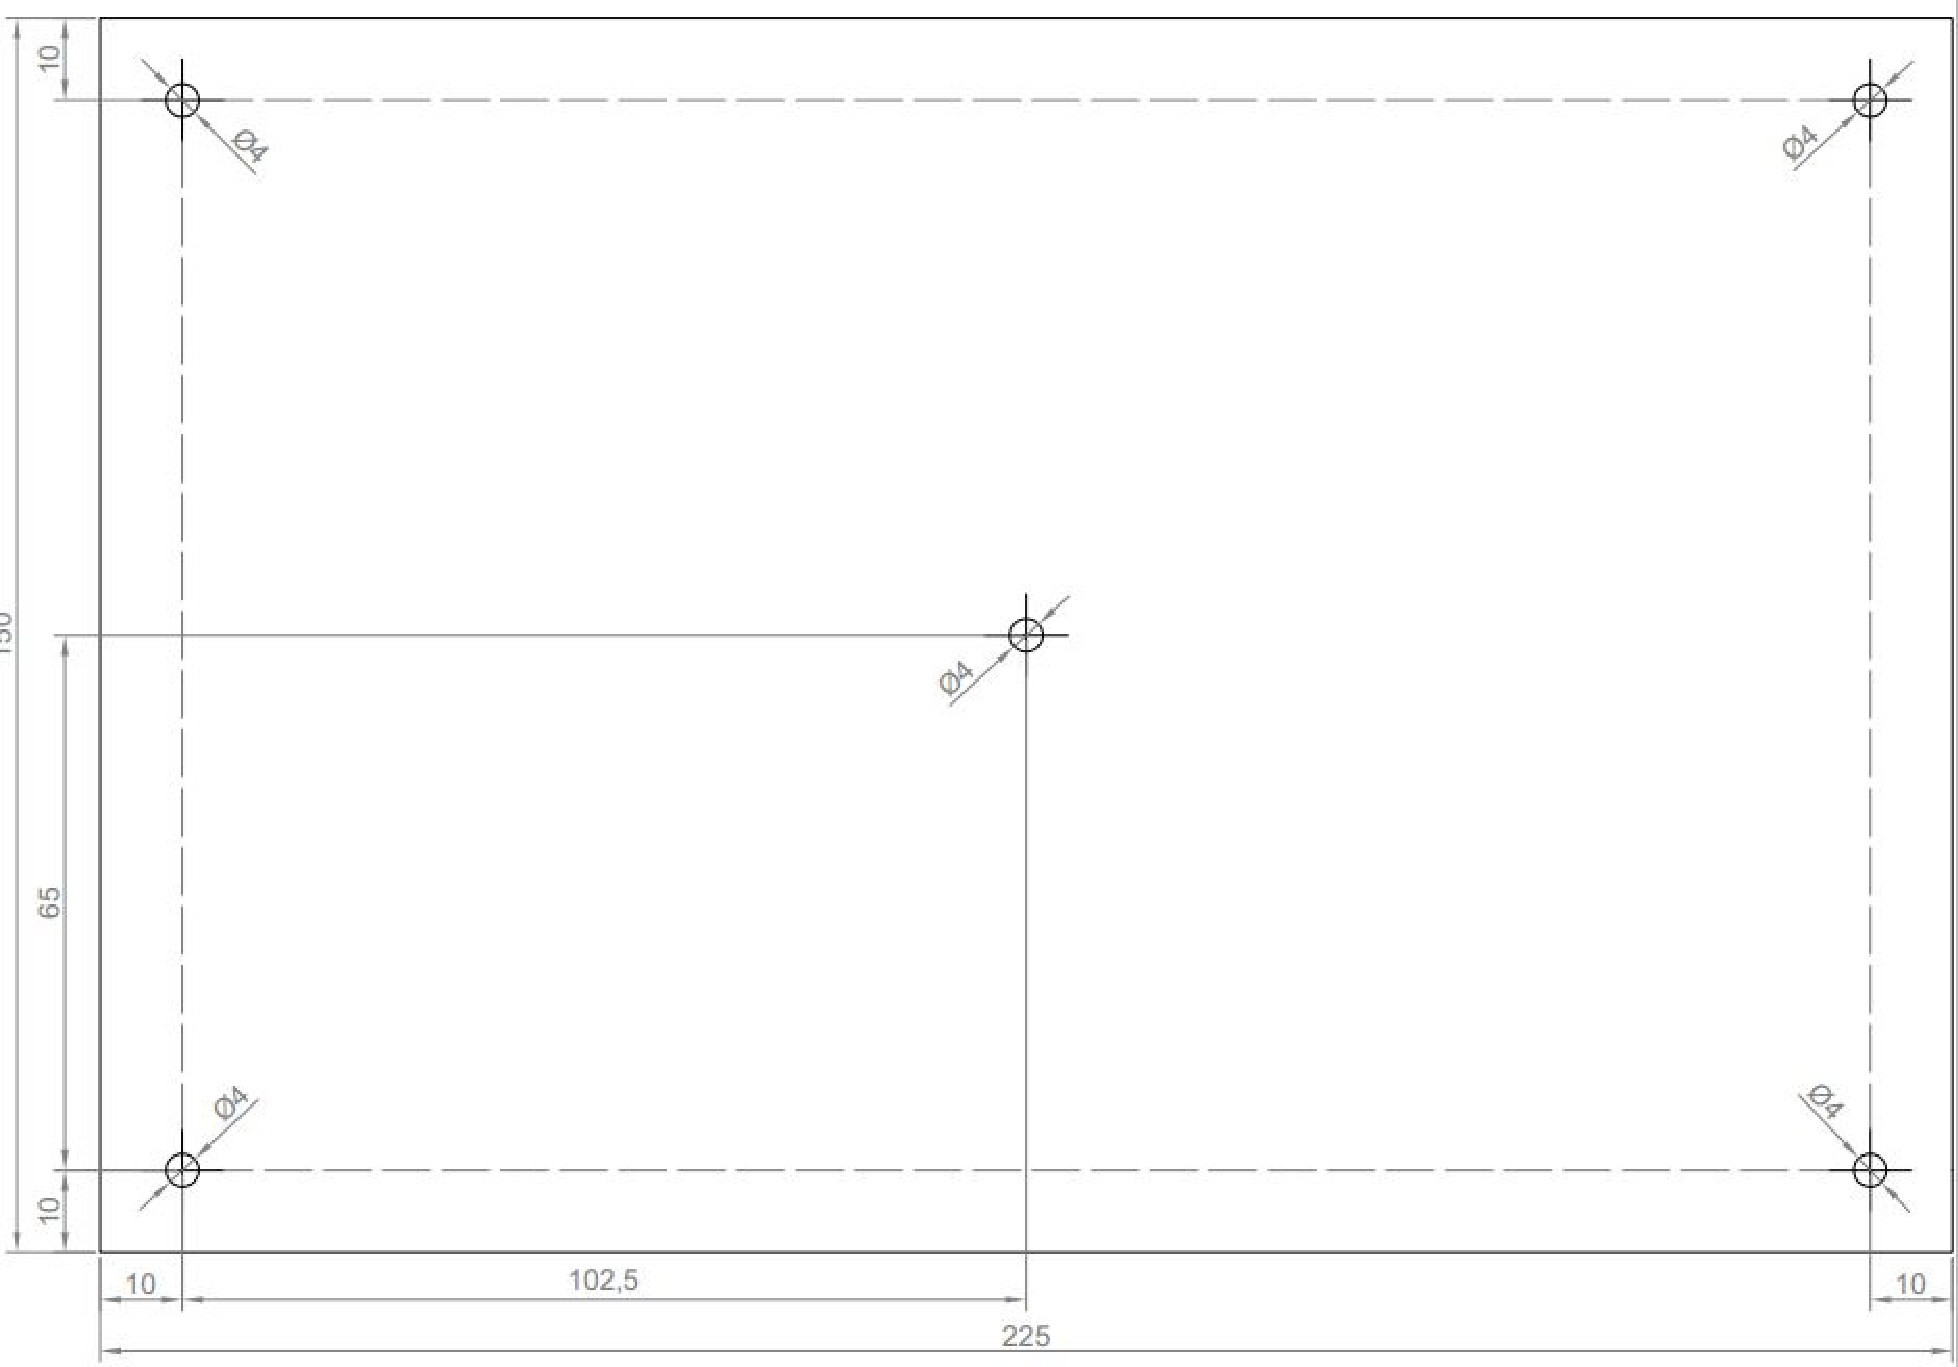
\includegraphics[width=1.00\textwidth]{Cad_Bodenplatte.pdf}
	\caption{CAD Zeichnung der Bodenplatte.}
	\label{fig:Cad_Bodenplatte}
\end{figure}

